\documentclass{beamer}

%---------- Theme & packages ----------
\usetheme{Madrid}
\usecolortheme{dolphin}
\usepackage[utf8]{inputenc}
\usepackage{physics, amsmath, amssymb}
\usepackage{caption}
\usepackage{graphicx}
\usepackage{tikz}
\usetikzlibrary{calc}
\usetikzlibrary{quantikz,fit}
\usepackage{yquant}
\useyquantlanguage{groups}
\usepackage{booktabs}    % for \toprule, \midrule, \bottomrule
\usepackage{hyperref}    % for \href links


%---------- Title data ----------
\title[Entanglement‑Efficient DQC]{Entanglement‑Efficient Bipartite‑Distributed Quantum Computing}
\author{Prepared by Gao Dingchao}
\institute{Reading Seminar}
\date{\today}

\AtBeginSection{
	\begin{frame}{Outline}
		\tableofcontents[currentsection]
	\end{frame}
}
%---------- Document ----------
\begin{document}
	
	% Title slide ---------------------------------------------------------
	\begin{frame}[plain]
		\titlepage
	\end{frame}
	
	\begin{frame}{References}
		\footnotesize
		\begin{thebibliography}{9}
			\bibitem{link} \href{https://pabloandrescq.github.io/}{Pablo Andres-Martinez, Senior R\&D Scientist at Quantinuum}
			\bibitem{wu2023}
			J‑Y. Wu \textit{et al.}, \emph{Entanglement‑efficient bipartite‑distributed quantum computing},\ Quantum \textbf{7} (2023).
%			\bibitem{ejpp}
%			J. Eisert \textit{et al.}, Phys. Rev.~A \textbf{62}, 052317 (2000).
		\end{thebibliography}
	\end{frame}
	
	% Outline slide --------------------------------------------------------
%	\begin{frame}{Outline}
%		\tableofcontents
%	\end{frame}
%	
	%---------------------------------------------------------------------
	\section{Background}
	
	\begin{frame}{Why Distributed Quantum Computing (DQC)?}
		\begin{itemize}
			\item \textbf{NISQ limitation:} single QPU constrained by qubit number, coherence, connectivity.
			\item \textbf{Connect QPUs via entanglement} \(\Rightarrow\) larger logical device.
			\item \textbf{Bottleneck:} entanglement distribution is costly \& probabilistic.
			\item Goal: \\[-.3em]
			\begin{block}{}
				Minimise \emph{EPR pairs} consumption for two‑party (bipartite) DQC while retaining universality.
			\end{block}
		\end{itemize}
	\end{frame}
	
	\begin{frame}{basic protocal}
		\begin{figure}
			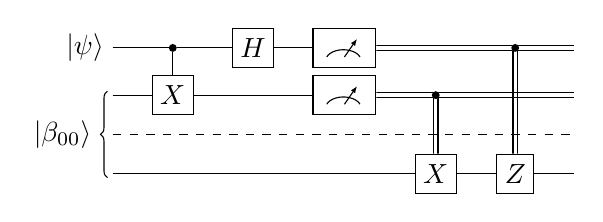
\begin{tikzpicture}
				\begin{yquant*}[operator/separation=5mm]
					qubit {$\ket{\psi}$} q;
					qubit {} Alice;
					nobit e;
					qubit {} Bob; 
					init {$\ket{\beta_{00}}$} (Alice, e, Bob);
					setstyle {dashed,thin} e;
					x Alice | q;
					h q;
					measure q,Alice;
					x Bob | Alice;
					z Bob | q;
				\end{yquant*}
			\end{tikzpicture}
			\caption{basic protocol for teleporting a qubit}
		\end{figure}
		\begin{equation*}
			\ket{\psi}\ket{\beta_{00}} \rightarrow \cdots
			\rightarrow \frac{1}{2}\left[\ket{00}\ket{\psi}+ \ket{01}X\ket{\psi}+\ket{10}Z\ket{\psi}+\ket{11}XZ\ket{\psi}\right]
		\end{equation*}
	\end{frame}
	
	\begin{frame}{Protocol in Distributed Quantum Operations}
		\centering
		% Top figure (main)
		\begin{minipage}{0.6\linewidth}
			\centering
			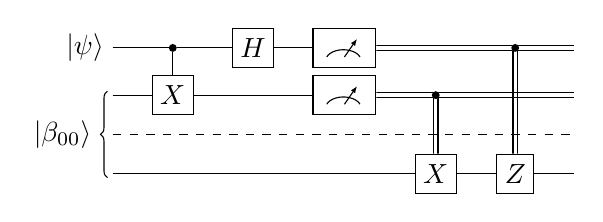
\begin{tikzpicture}
				\begin{yquant*}[operator/separation=5mm]
					qubit {$\ket{\psi}$} q;
					qubit {} Alice;
					nobit e;
					qubit {} Bob; 
					init {$\ket{\beta_{00}}$} (Alice, e, Bob);
					setstyle {dashed,thin} e;
					x Alice | q;
					h q;
					measure q,Alice;
					x Bob | Alice;
					z Bob | q;
				\end{yquant*}
			\end{tikzpicture}
%			\captionof{figure}{\textbf{Standard quantum teleportation.} Transfers an arbitrary qubit state to a remote party using entanglement and classical communication.}
		\end{minipage}
		
		\vspace{1em}
		
		% Bottom row: teledata and telegate side by side
		\begin{minipage}{0.48\linewidth}
			\centering
			\resizebox{\linewidth}{!}{
				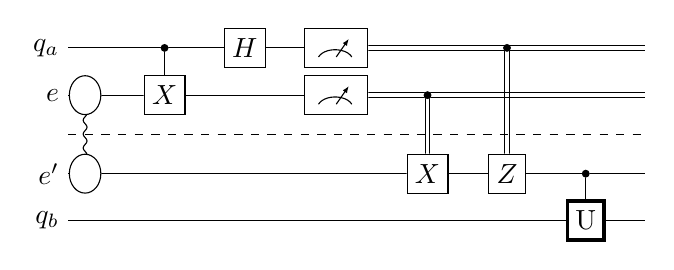
\begin{tikzpicture}
					\begin{yquant*}[operator/separation=5mm]
						qubit {$q_{a}$} a;
						qubit {$e$} Alice;
						qubit {} e;
						qubit {$e^\prime$} Bob;
						qubit {$q_{b}$} b;
						[operator/separation=-1pt,shape=yquant-circle] box {} (Alice, Bob);
						
						setstyle {dashed,thin} e;
						x Alice | a;
						h a;
						measure a,Alice;
						x Bob | Alice;
						z Bob | a;
						[very thick] box {U} b | Bob;
				\end{yquant*}
				\end{tikzpicture}
			}
			\captionof{figure}{\textbf{Teledata protocol.} The quantum state is first teleported, and then the operation \( U \) is applied on the remote system.}
		\end{minipage}
		\hfill
		\begin{minipage}{0.48\linewidth}
			\centering
			\resizebox{\linewidth}{!}{
				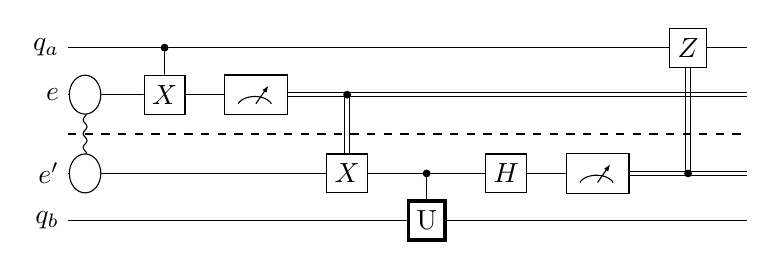
\begin{tikzpicture}
					\begin{yquant*}[operator/separation=5mm]
						qubit {$q_{a}$} a;
						qubit {$e$} Alice;
						qubit {} e;
						qubit {$e^\prime$} Bob;
						qubit {$q_{b}$} b;
						[operator/separation=-1pt,shape=yquant-circle] box {} (Alice, Bob);
						
						setstyle {dashed,thin} e;
						x Alice | a;
						measure Alice;
						x Bob | Alice;
						[very thick] box {U} b | Bob;
						h Bob;
						measure Bob;
						z a | Bob;
					\end{yquant*}
				\end{tikzpicture}
			}
			\captionof{figure}{\textbf{Telegate protocol.} The remote party applies a gate \( U \) using classical control based on measurement outcomes, without teleporting the quantum state.}
		\end{minipage}
	\end{frame}
	
	\begin{frame}{Newest Distributed Qubit Experiments (as of May 2025)}
		\scriptsize
		\begin{tabular}{@{}p{2.2cm}p{4.2cm}p{4.2cm}@{}}
			\toprule
			\textbf{Platform} & \textbf{Teledata} & \textbf{Telegate} \\ \midrule
			
			\textbf{Superconducting} 
			& \href{https://arxiv.org/abs/2302.08756}{64 m cryo-bus state teleportation, Qiu \emph{et al.}, 2025} 
			& \href{https://arxiv.org/abs/2407.16743}{\scriptsize99\% SWAP/CZ via detachable cable, Mollenhauer \emph{et al.}, 2025} \\
			
			\textbf{Trapped Ions} 
			& \href{https://www.nature.com/articles/s41534-024-00886-x}{14 km urban-fibre teleportation, Wang \emph{et al.}, 2024} 
			& \href{https://www.nature.com/articles/s41586-024-08404-x}{Teleported CZ \& Grover’s search (2 m), Main \emph{et al.}, 2025} \\
			
			\textbf{Neutral Atoms} 
			& \href{https://arxiv.org/abs/2504.05660}{420 km atomic-ensemble entanglement, Luo \emph{et al.}, 2025} 
			& Not yet demonstrated \\
			
			\bottomrule
		\end{tabular}
	\end{frame}
	\section{Problem in Telegate}
	
	\begin{frame}{The DQC Problem: Formal Definition}
		\textbf{Input:} Circuit $C$ on qubits $Q$, architecture graph $G=(V,E)$.
		
		\begin{itemize}
			\item Each module $A \in V$ has capacity $\omega(A)$ (data qubits) and $\varepsilon(A)$ (link qubits).
			\item Non-local gates (across modules) require 1 ebit each.
		\end{itemize}
		
		\textbf{Output:} A distribution $(\varphi, \tilde{C})$ such that:
		\begin{itemize}
			\item Qubit allocation map $\varphi: Q \rightarrow V$, $|\varphi^{-1}(A)| \le \omega(A)$.
			\item $\tilde{C}$ includes EPR pairs needs for each non-local gate.
			\item Active Pairs $\le \varepsilon(A)$ at all times.
		\end{itemize}
		
		\textbf{Goal:} Minimise total ebit usage.
	\end{frame}
	
	\begin{frame}{Two Key Subproblems in DQC}
		\begin{itemize}
			\item \textbf{Qubit Allocation: }
			\begin{itemize}
				\item Partition qubits across modules respecting $\omega(A)$.
				\item Minimise cut edges (i.e., potential non-local interactions).
			\end{itemize}
			\item \textbf{Non-local Gate Distribution:}
			\begin{itemize}
				\item find a way to implement the non-local gates
			\end{itemize}
		\end{itemize}
%		\textbf{1. Qubit Allocation}
%		\begin{itemize}
%%			\item Represent circuit as a hypergraph.
%			\item Partition qubits across modules respecting $\omega(A)$.
%			\item Minimise cut edges (i.e., potential non-local interactions).
%		\end{itemize}
%		
%		\vspace{0.3cm}
%		\textbf{2. Non-local Gate Distribution}
%		\begin{itemize}
%			\item Group cross-module gates into packets.
%			\item Embed intermediate operations to reduce ebit cost.
%			\item Assign packets to host modules using Steiner-tree or greedy heuristics.
%		\end{itemize}
	\end{frame}
	
%	\begin{frame}{some about gate}
%		Figure
%	\end{frame}
	
	\begin{frame}{TC vs. QCD: Key Differences}
		\begin{itemize}
			\item \textbf{Gate Types:} TC limits operations to those on-chip; QCD allows all, but nonlocal ones are costly.
			\item \textbf{Objective:} TC minimizes depth; QCD minimizes cross-QPU communication.
			\item \textbf{Optimization:} TC is local (gate-by-gate); QCD is global (qubit grouping).
			\item \textbf{Result:} TC outputs topology-compliant circuits; QCD allows nonlocal gates when needed.
		\end{itemize}
	\end{frame}
	
	\subsection{Qubit Allocation}
	
	\begin{frame}{Formal Restatement as Partitioning}
		\textbf{Interaction Graph:}
		\begin{itemize}
			\item Vertices: qubits $Q$.
			\item Edges: between $q_1$, $q_2$ if a two-qubit gate in $C$ involves them.
		\end{itemize}
		
		\textbf{Objective:} Partition $Q$ into $|V|$ disjoint sets
		\begin{itemize}
			\item Each set has size at most $\omega(A)$,
			\item Minimise the number of cut edges (gates across different sets).
%			\item (Opinion) load-balance: size of each set $\le (1+\delta)\frac{|V|}{k}$
		\end{itemize}
		This is a \textbf{capacity-constrained graph partitioning} problem.
	\end{frame}
	
	\begin{frame}{Main Partitioning Strategies}
		\begin{itemize}
			\item \textbf{Local Methods:}
			\begin{itemize}
				\item Iteratively improve an initial partition.
				\item Sensitive to starting configuration.
				\item Examples: Kernighan–Lin, Fiduccia–Mattheyses.
			\end{itemize}
			\item \textbf{Global Methods:}
			\begin{itemize}
				\item Use global graph properties to guide partitioning.
				\item Avoid arbitrary initialisation.
				\item Examples: Spectral Partitioning, Multilevel Partitioning.
			\end{itemize}
			\item \textbf{Simulated Annealing, ...}
		\end{itemize}
	\end{frame}
	
	
	\begin{frame}{Considerations in Practice}
		\begin{itemize}
			\item Partitioning quality affects EPR cost and circuit depth.
			\item Hardware-specific capacity limits must be respected.
			\item Gate commutativity can allow gate packet fusion before partitioning.
		\end{itemize}
	\end{frame}
	
	\begin{frame}{Definition: Hypergraph Partitioning}
		\textbf{Definition:} A hypergraph $G = (V, H)$ consists of a set of weighted vertices $V$ and a set of hyperedges $H$, where a hyperedge $h \subseteq V$ may connect more than 2 vertices.
		\vspace{1em}
		
		\textbf{Connectivity metric (\(\lambda - 1\))}:
		\[
		\lambda_G = \sum_{h \in H} ((\#\text{partitions containing endpoints of } h) - 1)
		\]
		
		The hypergraph partitioning problem is to find a balanced $k$-way partition minimizing this metric.
	\end{frame}
	
	\begin{frame}{Hypergraph Example}
		\begin{minipage}{0.48\linewidth}
			\centering
			\begin{figure}
				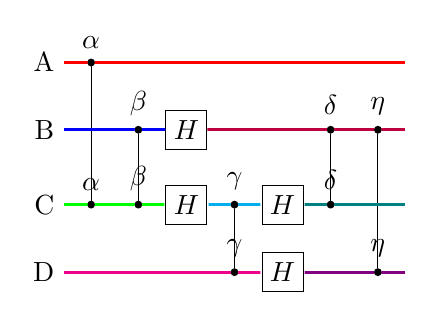
\begin{tikzpicture}
					\begin{yquant*}
						qubit {A} a;
						qubit {B} b;
						qubit {C} c;
						qubit {D} d;
						setstyle {very thick, red} a;
						setstyle {very thick, blue} b;
						setstyle {very thick, green} c;
						setstyle {very thick, magenta} d;
						["$\alpha$"]
						zz (a,c);
						["$\beta$"]
						zz (b,c);
						h b;
						setstyle {very thick, purple} b;
						h c;
						setstyle {very thick, cyan} c;
						["$\gamma$"]
						zz (c,d);
						h c;
						setstyle {very thick, teal} c;
						["$\delta$"]
						zz (b,c);
						h d;
						setstyle {very thick, violet} d;
						["$\eta$"]
						zz (b,d);
					\end{yquant*}
				\end{tikzpicture}
				\caption{Example quantum circuit, applying Hadamard gates H and CZ gates.}
			\end{figure}
		\end{minipage}
		\begin{minipage}{0.48\linewidth}
			\begin{figure}
				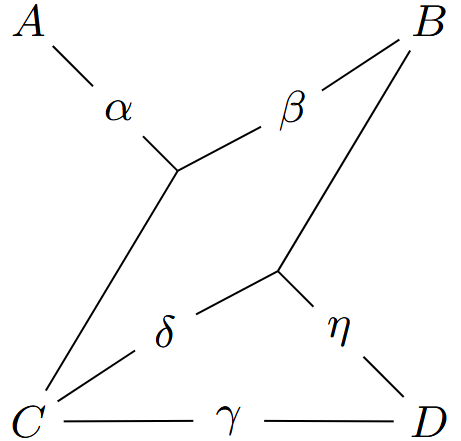
\includegraphics[width=.8\textwidth]{figures/hyper.png}
				\caption{hypergraph of the example circuit}
			\end{figure}
		\end{minipage}
	\end{frame}
	
	\begin{frame}{DQC and Hypergraph Mapping}
		\textbf{Correspondence between DQC and hypergraph partitioning:}
		\begin{center}
			\begin{tabular}{ll}
				\toprule
				\textbf{Hypergraph} & \textbf{DQC} \\
				\midrule
				Vertex & Qubits $\cup$ CRZ gates \\
				Hyperedge & Wire segment $\{q_i\} \cup \{g_1, \dots\}$ \\
				Vertex weight & 1 for qubits, 0 for CRZ \\
				$(\lambda - 1)$ metric & EPR cost \\
				Partitioning & Qubit allocation and gate execution \\
				\bottomrule
			\end{tabular}
		\end{center}
%		\vspace{1em}
%		\includegraphics[width=0.75\textwidth]{117a3058-c16a-4aa5-9c93-b84dec1e5cef.png} \
%		\tiny{Figure: Hypergraph derived from circuit (Fig. 5, Andres-Martinez et al.)}
	\end{frame}
	
	\begin{frame}{Why Hypergraph, Not Graph?}
		\begin{itemize}
			\item Graph cut counts \textit{each gate} separately.
			\item Hypergraph cut counts \textit{each packet} once.
			\item Captures the cost structure of shared EJPPs (ebit sharing).
		\end{itemize}
		\begin{minipage}{.3\linewidth}
			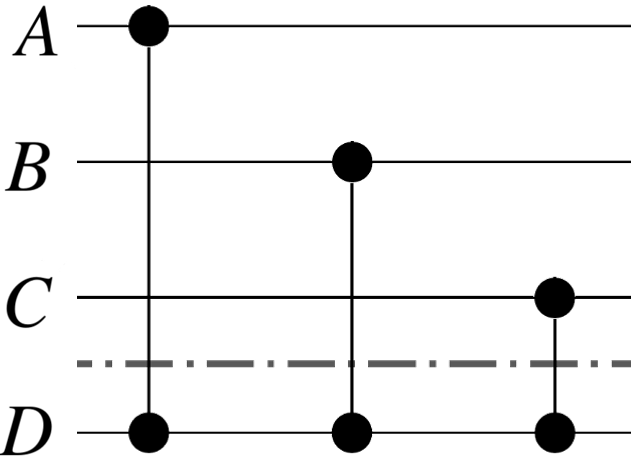
\includegraphics[width=.9\textwidth]{figures/why1.png}
			\captionof{figure}{An example circuit}
		\end{minipage}
		\begin{minipage}{.3\linewidth}
			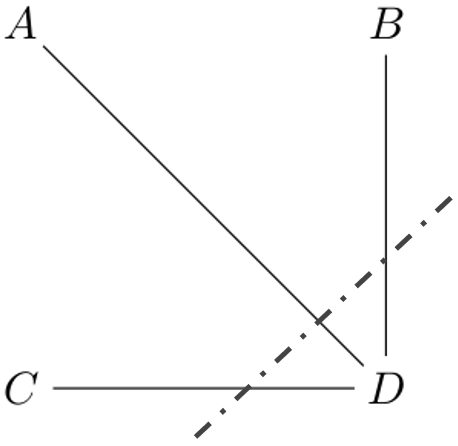
\includegraphics[width=.9\textwidth]{figures/why2.png}
			\captionof{figure}{\textbf{Graph}: This partition shown cuts three edges}
		\end{minipage}
		\begin{minipage}{.3\linewidth}
			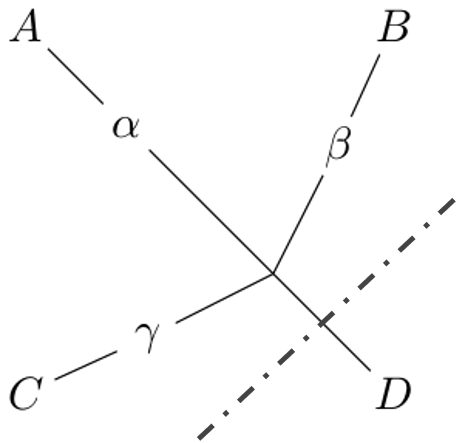
\includegraphics[width=.9\textwidth]{figures/why3.png}
			\captionof{figure}{\textbf{Hypergraph}: This partition shown cuts One edges}
		\end{minipage}
	\end{frame}
	
	%------------------------------------------------------
	\begin{frame}{Key Result}
		\begin{block}{Theorem}
			For fully connected networks,
			\begin{itemize}
				\item Each valid distribution $\Rightarrow$ a hypergraph partition
				\item If the circuit’s hypergraph can be partitioned cutting n edges, the circuit can be distributed using n ebits.
				\item \textit{Optimal partition} $\Leftrightarrow$ \textit{Minimum ebit allocation}
			\end{itemize}
		\end{block}
	\end{frame}
	
	%------------------------------------------------------
	\begin{frame}{Qubit Allocation Workflow Summary}
		\begin{enumerate}
			\item Rebase circuit to \{H, RZ, CRZ\}
			\item Construct hypergraph (qubit/gate vertices, one edge per packet)
			\item Use hypergraph partitioner (e.g. KaHyPar) with capacity constraints
			\item Read module assignment from partition
		\end{enumerate}
		\vspace{0.5em}
		\textbf{Ebit count = Hypergraph cut cost}
	\end{frame}
	
	\subsection{Gate Distribution}
	%	need hypergraph
	\begin{frame}{Recall protocol}
		\begin{columns}[T]
			\column{0.58\textwidth}
			Controlled‑unitary \(CU\) can be implemented non‑locally with \textbf{one ebit} using:
			\begin{itemize}
				\item \emph{Starting process}: cat‑entangler.
				\item \emph{Kernel}: local $C_{e,U}$.
				\item \emph{Ending process}: cat‑disentangler.
			\end{itemize}
			\column{0.4\textwidth}
			\centering
			% Fig. 1 of the paper
			\begin{figure}
				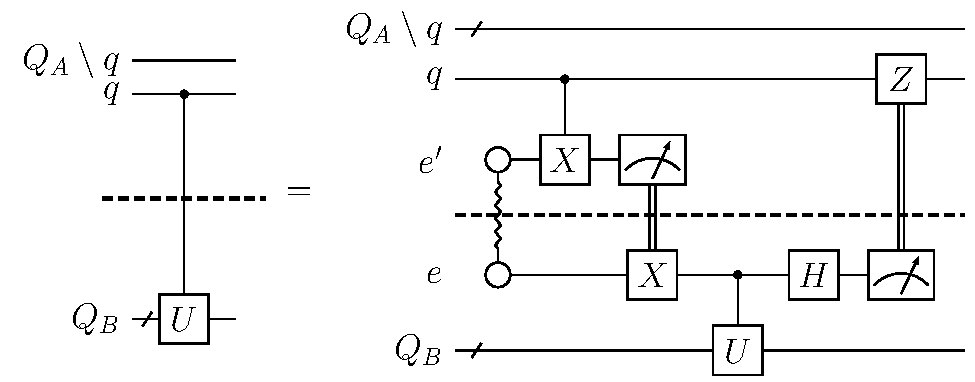
\includegraphics[width=\linewidth]{figures/EJPP_protocol.pdf}
				\caption{Telgate protocol}
			\end{figure}
		\end{columns}
	\end{frame}
	%------------------------------------------------------
	\begin{frame}{Setting the Stage}
%		After hypergraph partitioning we know \emph{where} each logical qubit resides.  Any CRZ acting on qubits in different modules becomes a \textbf{non‑local gate} that must be executed over the network.
		
%		\vspace{1em}
		Goal of gate distribution: realise every non‑local gate while \emph{minimising entanglement (ebit) cost}.  
		\begin{figure}
			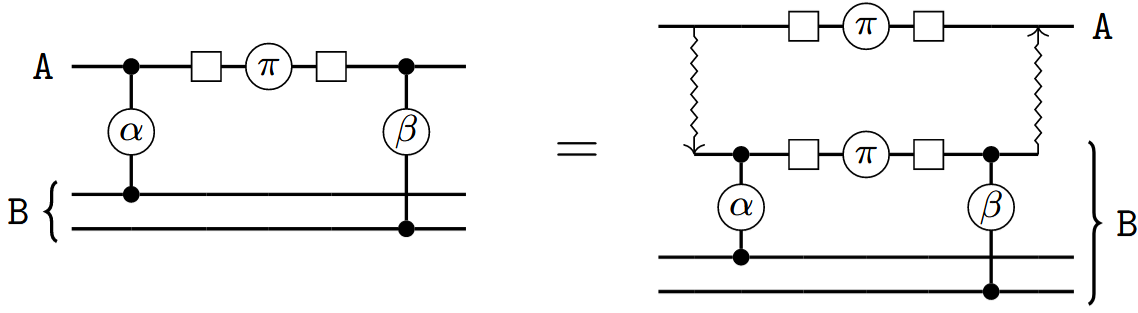
\includegraphics[width=.8\textwidth]{figures/emb.png}
			\caption[]{Examples of EJPP Protocol}
		\end{figure}
	\end{frame}
	
	
	%------------------------------------------------------
%	\begin{frame}{Why Extend the Original Protocol?}
%		Original simultaneous‑teleportation realises \emph{one} gate per ebit.
%		
%		\vspace{0.5em}
%		\textbf{EJPP advantages}
%		\begin{itemize}
%			\item \textbf{Cost leverage}: $m$ gates \(\Rightarrow\) 1 ebit instead of $m$ ebits.
%			\item \textbf{Local corrections}: Pauli corrections confined to the two modules.
%			\item \textbf{Entanglement reuse}: required for Steiner‑tree optimisation.
%		\end{itemize}
%	\end{frame}
	
	\begin{frame}{Distributing and Embedding Processes}
		\begin{block}{Definition: Distributing Process}
			A unitary $U$ is \emph{q‑rooted distributable} if it is diagonal/antidiagonal in $q$ and decomposes as
			$U = \sum_{ij} \Delta_{ij}\,|i\rangle\!\langle j|_q\,\otimes V_j\otimes W_j$.
			\begin{itemize}
				\item Implementable with \textbf{one ebit} (extends EJPP).
			\end{itemize}
		\end{block}
		\vspace{.5em}
		\begin{block}{Definition: Embedding Process}
			A unitary $U$ is \emph{q‑rooted embeddable} if
			$C_{q,X_e}\,U\,C_{q,X_e} = (L_A\otimes L_B)\,U\,(K_A\otimes K_B)$.
			\begin{itemize}
				\item Enables merging of non‑sequential distributing gates.
			\end{itemize}
		\end{block}
	\end{frame}

	
	\begin{frame}{Merging Packing Processes}
		\textbf{Statement:}
		If $P_{q,e}[K_1]$ and $P_{q,e}[K_2]$ are packing processes implementing $U_1$ and $U_2$ respectively, then
		\[
		U_2U_1 = P_{q,e}[K_2K_1]\quad\text{(still 1 ebit)}.
		\]
		\pause
		\begin{block}{Implication}
			Sequential or \emph{merged‑via‑embedding} distributable gates can share \textbf{one} entangled pair.
		\end{block}
	\end{frame}
	
	%\subsection{Graph Representation}
	
%	\begin{frame}{Packing Graph}
%		\begin{itemize}
%			\item \textbf{Vertices:} distributable nodes $(q,t)$.
%			\item \textbf{Edges:} exist if intervening gates are embeddable \(\Rightarrow\) \emph{packable}.
%			\item Connected vertices form a \textbf{distributable packet} implemented with one packing process.
%		\end{itemize}
%		%\includegraphics[width=0.8\linewidth]{fig_packet_graph.png}
%		%\captionof{figure}{Schematic packing graph.}
%	\end{frame}
	
	\begin{frame}{Conflict Graph and Edge Types}
		\begin{itemize}
			\item \textbf{Vertices:} indecomposable packing kernels (`D` for distribute, `B` for embed).
			\item \textbf{Edges:}
			\begin{description}
				\item[DD‑type] intrinsic conflict between two distributing options.
				\item[DB‑type] extrinsic resource conflict distribute vs embed.
				\item[BB‑type] embed vs embed (resource or structural).
			\end{description}
		\end{itemize}
		\begin{figure}
			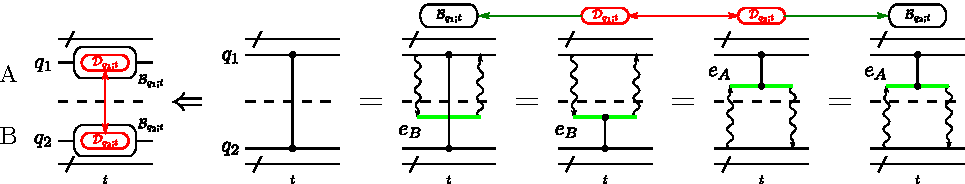
\includegraphics[width=.9\linewidth]{figures/conflict_DD_intrinsic.pdf}
			\caption{DD‑type conflict example.}
		\end{figure}
	\end{frame}
	
	
	%------------------------------------------------------
	\begin{frame}{Steiner‑Tree Entanglement Routing}
		\begin{itemize}
%			\item In sparse or heterogeneous topologies two modules may lack a direct link.
			\item Prepare Bell pairs only along the edges of the \textit{minimum Steiner tree} connecting the two modules.
			\item Keep the tree\,'s entanglement \emph{alive} for the whole packet \(\Rightarrow\) edges are created once, then reused.
		\end{itemize}
		\begin{center}
			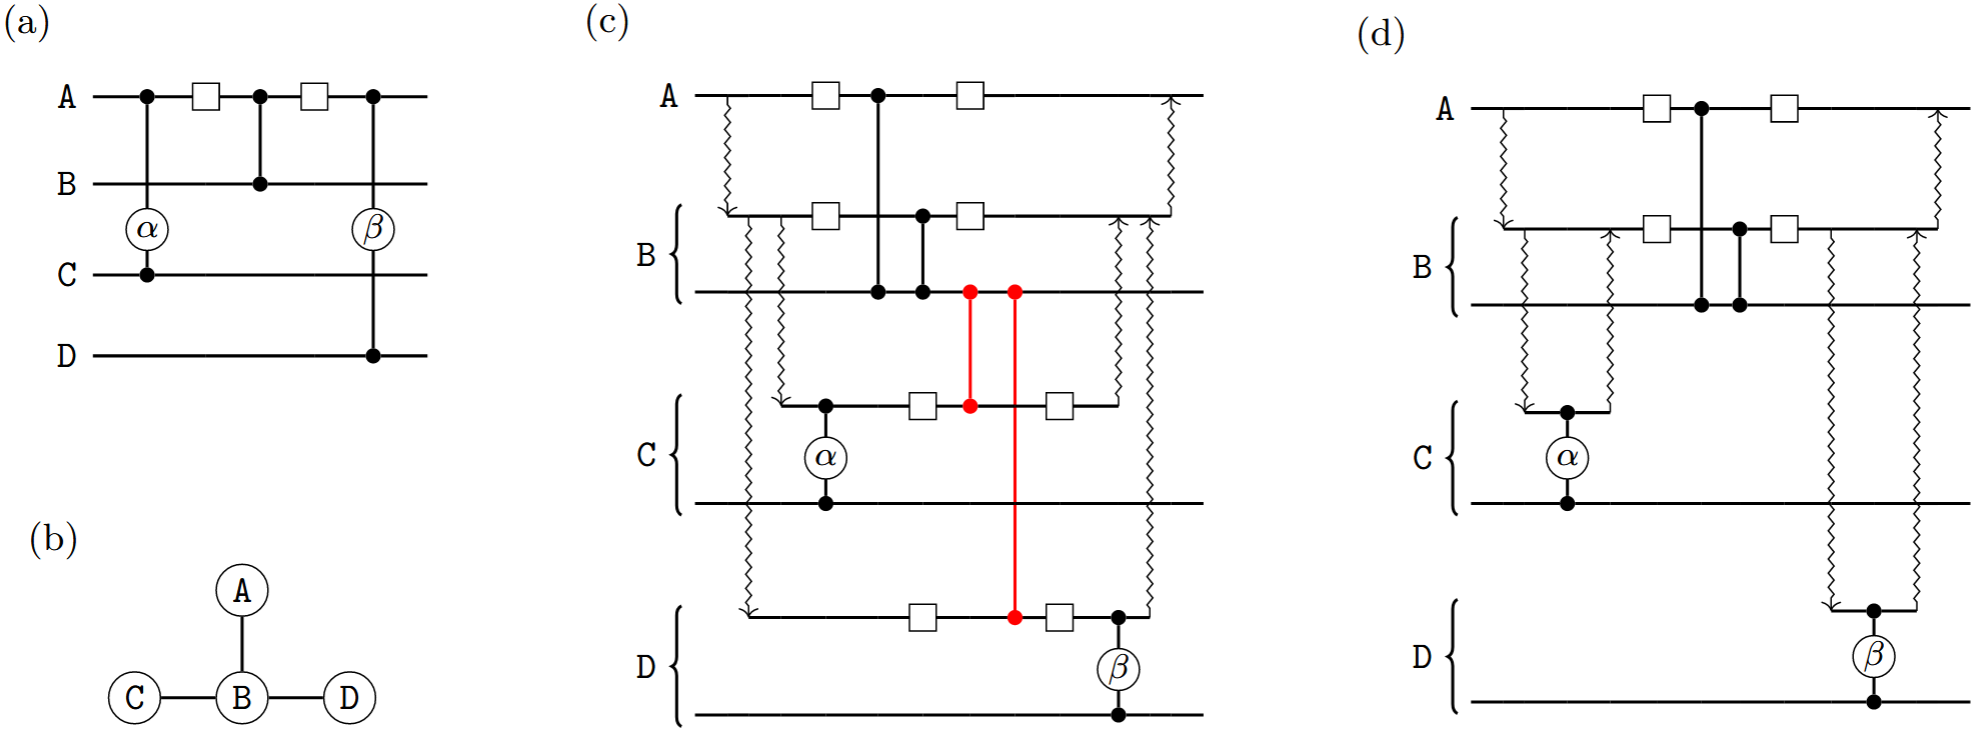
\includegraphics[width=0.9\textwidth]{figures/tree.png}
			\captionof{figure}{Steiner tree Example}
		\end{center}	
	\end{frame}
	%------------------------------------------------------
	\begin{frame}{End‑to‑End Workflow}
		\begin{enumerate}
			\item \textbf{Allocate qubits} via hypergraph partitioning.
			\item \textbf{Group non‑local CRZs} on each root into packets.
			\item For each packet:
			\begin{enumerate}
				\item Find Steiner tree between the two modules.
				\item Execute packet using \textbf{EJPP} over that tree.
			\end{enumerate}
			\item Apply \textbf{embedding} and \textbf{detached} rewrites when profitable.
		\end{enumerate}
		\vspace{1em}
		\alert{Result}: full distributed circuit with (near‑)minimal ebit count.
	\end{frame}
	
	\section{WIP}
	\begin{frame}{Quantum Fourier Transform (4‑Qubit Example)}
		\begin{figure}
			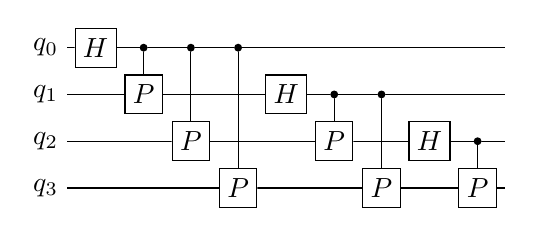
\begin{tikzpicture}
				\begin{yquant*}
					qubit {$q_{\idx}$} q[4];
					h q[0];
					box {$P$} q[1] | q[0];
					box {$P$} q[2] | q[0];
					box {$P$} q[3] | q[0]; 
					h q[1];
					box {$P$} q[2] | q[1];
					box {$P$} q[3] | q[1];
					h q[2];
					box {$P$} q[3] | q[2];
				\end{yquant*}
			\end{tikzpicture}
			\caption[]{Example 4‑qubit QFT circuit. Controlled‑phase gates $P_{\theta}$ apply $|1\rangle\!\langle 1|\otimes e^{i\theta Z}$.}
		\end{figure}
	\end{frame}
	
	\begin{frame}{Static $k$‑Partition Scheme}
		\begin{figure}
			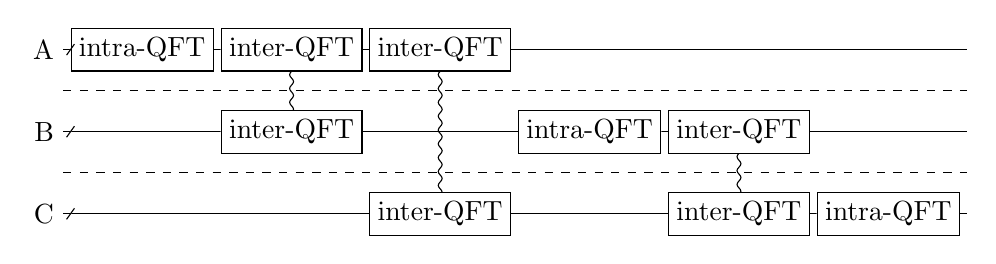
\begin{tikzpicture}
				\begin{yquant*}
					qubit {A} a;
					qubit {} s0;
					qubit {B} b;
					qubit {} s1;
					qubit {C} c;
					slash a;
					slash b;
					slash c;
					setstyle {dashed,thin} s0;
					setstyle {dashed,thin} s1;
					box {intra-QFT} a;
					box {inter-QFT} (b,a);
					box {inter-QFT} (c,a);
					box {intra-QFT} b;
					box {inter-QFT} (c,b);
					box {intra-QFT} c;
					
				\end{yquant*}
			\end{tikzpicture}
			\caption[]{Illustration of a 3‑partition mapping of the 4‑qubit QFT.}
		\end{figure}
	\end{frame}
	
	\begin{frame}{With Mid‑Circuit Measurements}
		\begin{figure}
			\resizebox{.9\textwidth}{!}{
				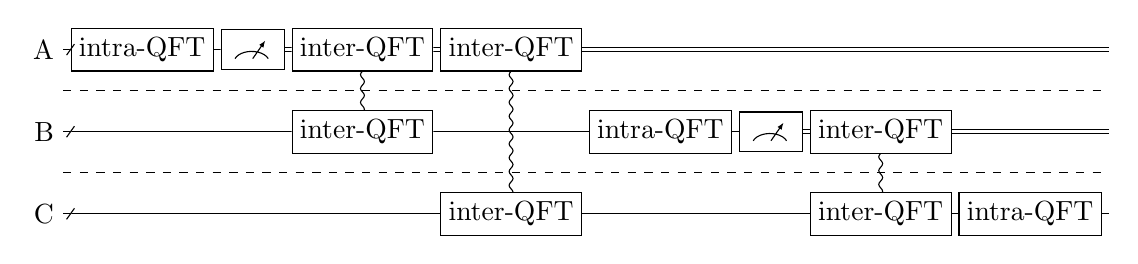
\begin{tikzpicture}
					\begin{yquant*}
						qubit {A} a;
						qubit {} s0;
						qubit {B} b;
						qubit {} s1;
						qubit {C} c;
						slash a;
						slash b;
						slash c;
						setstyle {dashed,thin} s0;
						setstyle {dashed,thin} s1;
						box {intra-QFT} a;
						measure a ;
						box {inter-QFT} (b,a);
						box {inter-QFT} (c,a);
						box {intra-QFT} b;
						measure b;
						box {inter-QFT} (c,b);
						box {intra-QFT} c;
						
					\end{yquant*}
				\end{tikzpicture}
			}
			\caption[]{Dynamic variant: measurement outcomes on partitions A and B classically steer subsequent inter‑partition operations.}
		\end{figure}
	\end{frame}

\end{document}
